\documentclass[prl,amsmath,amssymb,floatfix,superscriptaddress,notitlepage,twocolumn]{revtex4}
\usepackage{algorithm2e}
\usepackage{graphicx, tikz}
\usepackage{hyperref}
\usepackage{bm}
\usepackage{amssymb}
\usepackage{xifthen}
\usepackage{color}
\usepackage{datetime}
\usepackage{float}
\usepackage{bm}
\usepackage{changepage}
\usepackage{bbold}
\usepackage{multirow}
\usepackage{algorithm}
\usepackage{algpseudocode}

%\usepackage{caption}


%editing commands for the users in our group (You can make more)
\newcommand{\Damian}[1]{\textcolor{magenta}{(Damian: #1)}}
\newcommand{\Alec}[1]{\textcolor{blue}{(Alec: #1)}}
\newcommand{\Jack}[1]{\textcolor{green}{(Jack: #1)}}
\newcommand{\Rawan}[1]{\textcolor{red}{(Rawan: #1)}}


%commands to make math expressions easier
\newcommand{\ee}[1]{\begin{align} #1 \end{align}} 						%align environment
\newcommand{\vc}[1]{\vec{\mathbf{#1}}} 								%arrowed bold vector
\newcommand{\intg}[2]{\int \! \mathrm{d}^{#1}\vc{#2} \ }					%integral with measure
\newcommand{\nn}[1][]{\ifthenelse{\isempty{#1}}{\nonumber \\}{\nonumber}}	%nonumber shortcut
\newcommand{\dv}{\partial }											%partial derivative shortcut
\newcount\colveccount												%column vector
\newcommand*\colvec[1]{
        \global\colveccount#1
        \begin{bmatrix}
        \colvecnext
}
\def\colvecnext#1{
        #1
        \global\advance\colveccount-1
        \ifnum\colveccount>0
                \\
                \expandafter\colvecnext
        \else
                \end{bmatrix}
        \fi
}



\begin{document}

\title{Percieving Circadian Gene Expression through Artificial Neural Networks}

\author{Damian Sowinski}
\email{Damian.Sowinski@dartmouth.edu}
\affiliation{Center for Cosmic Origins \\Department of Physics and Astronomy, Dartmouth College}

\author{Alexander Crowell}
\email{Alexander.M.Crowell@dartmouth.edu}
\affiliation{Department of Genetics, Geisel School of Medicine, Dartmouth College}

\author{Jack Holland}
\email{Jack.E.Holland@dartmouth.edu}
\affiliation{Department of Computer Science, Dartmouth College,Hanover, NH 03755, USA}

\author{Rawan Al Ghofaili}
\email{Rawan.al.Ghofaili@dartmouth.edu}
\affiliation{Department of Computer Science, Dartmouth College,Hanover, NH 03755, USA}


\date{Last Updated: \today, \currenttime}

\begin{abstract}

The circadian clock regulates many critical processes, notably including metabolism and cancer suppression.  In order to improve both our understanding of the clock and drug discovery and delivery for the many disease processes it interacts with the ability to accurately classify genes as circadianly regulated based on expression data is critical.  To improve on existing classification of circadian gene expression we employed an artificial neural network and compared it's performance to the current standard algorithm $JTK_{CYCLE}$.  We employ a feed forward network, and examine the architectural constraints to optmize the ability of the network to classify circadian experession. We discuss the theoretical construction of an artificial neural network (ANN) to better understand design choices made in this work. Preliminary results are found and possible modifications to the network are discussed.

\end{abstract}

\maketitle


\section{Circadian Rhythms}
Circadian Clocks are an adaptive response to the evolutionary necessity of anticipating day night cycles.  They occur widely in higher eukaryotes and sparsely in fungi and cyanobacteria.  Because of the widespread and longstanding evolutionary history of organisms specializing their activity to a specific phase of the day night cycle, circadian clocks, where present, have been found to regulate almost every biological process imaginable.  Notable among these are the cell cycle, DNA damage repair and metabolism, processes central to the majority of human disease \cite{Dunlap99}.  Perturbation of the clock upsets these processes as well and has been shown to contribute to disease \cite{Bass10}.  One of the most important recent trends in circadian research has been the interaction of the circadian cycle with disease treatment, specifically the timed delivery of medicine \cite{Zhang14}.  Additionally the circadian clock's modulation of such a wide variety of gene and protein expression along with the diverse processes employed to achieve that modulation provides an excellent opportunity for the study of gene regulation at every stage from transcription to degradation \cite{Mehra09,Menet14}.

The current state of the art in the identification of Circadian gene expression is the JTK\_CYCLE algorithm (JTK) \cite{Hughes10}.  JTK uses a nonparametric test for monotonic orderings in the data over all possible period lengths and phases and for high (\~2hr) resolution data it provides high sensitivity, specifity and computational efficiency.  JTK and earlier approaches including curve fitting \cite{Straume04}, autocorrelation \cite{Levine02}, Fourier analysis \cite{Wichert04,Whitfield04} and Fisher's G Test \cite{Wichert04} all fall short however as the resolution of data decreases.  Due to technical challenges in the maintenance and synchronization of cells as well as sequencing costs, dataset resolution is currently a major limiting factor in the identification of circadian genes.  Therefore an improved computational technique for identifying circadian genes in low temporal resolution data could rapidly provide knew knowledge from publicly available pre-existing datasets

\section{Artificial Neural Networks}
In this section we go over the theoretical background of how to build an ANN, develop the formalism behind the backpropogation algorithm, and discuss possible candidates for tunable hyperparameters/functions used. We will develop both the feed forward and back prop algorithms for completeness. 

ANNs are a supervised machine learning algorithm used for classification problems. Given some labeled set of data $\mathcal{D}=\{(\vc x,\vc y)_i\}_{i=1}^D$, where to each multidimensional datum $\vc x$ there is an associated multidimensional label $\vc y$, the ANN learns from $\mathcal{D}$ how to place labels on new data. Processing a datum by the network is accomplished via the \textit{feed forward} algorithm, while training is done through the \textit{back propogation} algorithm. 

The basic building block of an ANN is the perceptron. $N$ signals go into the perceptron, are weighted, summed, and then put through some activation function to create an output signal:
\ee{
\label{perceptron}
\text{output}=\theta(\sum_{i=0}^{N}w_i\times\text{input}_i)
}
The form of the \textbf{activation function}, $\theta$ is typcally chosen to be one that gives a value of $1$ for arguments larger than some threshhold, and $0$ otherwise. The backpropogation algorithm requires this function to be both differentiable and invertible, so typical choices include the logistic, arctan, and hyperbolic tangent functions. Note also that the sum begins at $0$, leading to $N+1$ inputs. The $0^{th}$ input is always taken to be $1$, and its corresponding weight is known as the \textbf{bias}.

We can stack perceptrons into layers, and in turn stack those together so that the inputs of the $l^{th}$ layer are the outputs coming from the $(l-1)^{th}$ layer. This is the basic form of an ANN. We need only specify the architecture of the ANN (number of layers/\{Input dimensionality,number of perceptrons in each layer\}), which will be $L/\{N_0,N_1,\dots,N_L\}$. Note that $N_0$ represents the dimensionality of the input signal, and $N_L$ is the dimensionality of the output layer. Between each pair of layers there is a corresponsing weight matrix, $\textbf{w}^{(l)}:\mathbb{R}^{N_{l-1}}\rightarrow\mathbb{R}^{N_l}$, the components of which are $w_{ij}^{(l)}$, where $l$ is the target layer, $i$ is the index of the \textit{to} perceptron in the target layer, and $j$ is the \textit{from} perceptron in the domain layer. We denote the set of all these matrices \textbf{W}, and refer to this set as the \textbf{architecture} of our ANN. With these definitions in hand, we can write the output of the $i^{th}$ perceptron in the $l^{th}$ layer in compact form:
\ee{
x^{(l)}_i=\theta(\sum_{j=0}^{N_{l-1}}w^{(l)}_{ij}x^{(l-1)}_j)
}
where once again,, the $w^{(l)}_{i0}$'s represent biases. 

With the architecture in place, we can now easily state the feed forward algorithm, \ref{feed_forward}. It is nothing more than allowing an input signal propagate through the network, and eventually pop out at the end.

This is all fine and dandy, but what we want is to be able to train the network based on the known labels. We need to compare the output of the network with the known label, define an error based on that comparison, and then alter the weights in the network so as to decrease that error. Furthermore, when the weights are changed, we do not want them to take on any values (one can imagine one weight becoming so high that it dominates the flow of signals in the ANN), so we must also regularize the way in which the error function is causing the weights to change. These statements can be made more precise.

Initialize an ANN with randomized weights. Take a datum $(\vc x^{(0)},\vc y)$ and have the ANN process the input to get an output $(\vc x^{(L)},\vc y)$. We define the cost of the function as an explicit function of the output, the \textbf{error}, and an explicit function of the weights, the \textbf{regularizer}:
\ee{\label{CostFactorization}
C(\vc x^{(L)},\vc y,\textbf{W})=E(\vc x^{(L)},\vc y)+R(\textbf{W})
}
This factorization of the arguments is a bit deceptive, since the output is an implicit function of the weights of the network. This fact will be crucial as we start exploring weight-space and will need to take gradients of the cost with respect to the weights. Our goal will be to decrease the cost of our ANN at each iteration by changing the weights of the network. Over the course of many epochs, the network will learn the patterns in the data, and we will have minimized the cost. So, how do we choose the change in weights to achieve this at each iteration?

We want:
\ee{
C(\vc x^{(L)},\vc y,\textbf{W}+\delta\textbf{W})\le C(\vc x^{(L)},\vc y,\textbf{W})\nn[1]
}
Expanding the RHS to first order in $\delta\textbf{W}$ we have:
\ee{
\nabla C\cdot \delta\textbf{W}\le0\nn[1]
}
where the gradient is taken with respect to the weights. We can easilly satisfy this equation if we choose:
\ee{
\label{LearningRule}
\delta\textbf{W}&=-\eta \nabla C\nn
\Downarrow&\nn
\delta w^{(l)}_{ij}&=-\eta\frac{dC}{d w^{(l)}_{ij}}
}
This is our \textbf{learning rule}. The hyperparameter $\eta$ is called the \textbf{learning rate}. Taking the gradient of the regularizer is simple, since it is an explicit function of the weights. To take the gradient of the error, however, we will have to employ some mathematical trickery. We have to use the fact that the output depends on the weights, making the error an implicit function of the weights. 

First off we will break up the reweighing of the ANN layer by layer. So we will start at the output layer, and move backward. To proceed we need one result on how to differentiate an output neuron with respect to weight:
\ee{
\frac{d x^{(l)}_n}{d w^{(l)}_{ij}}=&\frac{d}{d w^{(l)}_{ij}} \theta(\sum_{k=0}^{N_{l-1}}w^{(l)}_{nk}x^{(l-1)}_k)\nn
=&\theta'\circ\theta^{-1}(x^{(l)}_n)\delta_{ni}x^{(l-1)}_j
}
if we define $\phi=\theta'\circ\theta^{-1}$, the gradient of the error can then be written:
\ee{
\frac{d E}{d w^{(L)}_{ij}}=&\sum_{k=1}^{N_L}\frac{\dv E}{\dv x_k^{(L)}}\frac{d x^{(l)}_k}{d w^{(l)}_{ij}}\nn
=&\frac{\dv E}{\dv x_i^{(L)}}\phi(x_i^{(L)})x_j^{(L-1)}
}
We can generalize this for the gradient w.r.t. other layer weights by defining:
\ee{
\delta_i^{(l)}=\left\{
\begin{array}{lr}
       \phi(x_i^{(l)})\frac{\dv E}{\dv x_i^{(l)}} & l=L\\
       \phi(x_i^{(l)})\sum_j\delta^{(l+1)}_jw^{(l+1)}_{ji} & l<L
\end{array}
\right.
}
This is known as the $\delta$-rule, and is used to write the learning rate in its compact form:
\ee{
\delta w^{(l)}_{ij}=-\eta\left(\frac{dR}{d w^{(l)}_{ij}}+\delta^{(l)}_ix^{(l-1)}_j\right)
\frac{d E}{d w^{(L)}_{ij}}=&\sum_{k=0}^{N_L}
}
Take a datum $(\vc x^{(0)},\vc y)$ and process the input to get an output $d=(\vc x^{(L)},\vc y)$. Then determine the cost of this processed output and the weights of the network via:
\ee{
C=C((\prod_l\theta\circ \textbf{W}^{(l)})(\vc{x}^{(0)}),\vc{y},\textbf{W})
}
This is all we need to define the back propogation algorithm, \ref{back_prop}.


To go any farther we need to discuss the possible choices for the functions that define our network: the activation, error, and regularizer. We will now discuss each of these in turn. 

\subsection{Function Choices}
\subsubsection{Activation Function}
The only constraints that we have on our choice is that the function be both differentiable and invertible. Typical choices are therefore any smooth strictly monotonic function. We should also specify the domain of the inputs. The list below has been normalized to the range $(0,1)$, and we have included the backprop functions for completeness:
\begin{itemize}
\item Sigmoid (blue)
\ee{
\theta(x)=&\frac{1}{1+e^{-x}}\\
\phi(x) =& x(1-x)\nn[1]
}
\item Hyperbolic Tangent (magenta)
\ee{
\theta(x) =& \frac{1}{2}(1+\text{tanh} x)\\
\phi(x) =& 2x(1-x)\nn[1]
}
\item Arctangent (gold)
\ee{
\theta(x) =& \frac{1}{2}(1+\frac{2}{\pi}\text{arctan} x)\\
\phi(x) =& \frac{1}{\pi}\cos^2\frac{\pi}{2}(2x-1)\nn[1]
}
\end{itemize}

The activations are plotted in figure \ref{AF}. The qualitative differences are mostly with the arctan function, which requires incredibly high absolute value inputs to generate output close to $0$ or $1$. The corresponding backprop functions are plotted in figure.

\begin{figure*}[ht!]
\label{AF}
\centering
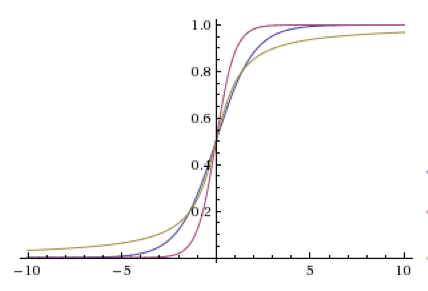
\includegraphics[width=0.48\textwidth]{ActivationFunctions.png}\hfill
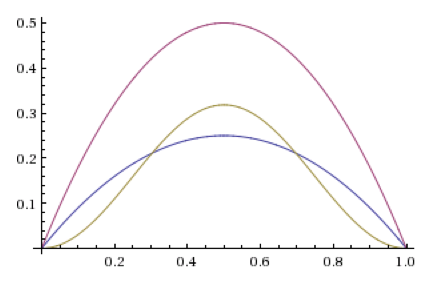
\includegraphics[width=0.48\textwidth]{BackPropActivationFunctions.png}
\caption{On the left we have the activation functions plotted, and the back propagated functions on the right. The sigmoid, hyperbolic tangent, and arctangent are blue, magenta, and gold, respectively. Not that the main difference }
\end{figure*}

The activations are plotted in figure \ref{AF}. The qualitative differences are mostly with the arctan function, which requires incredibly high absolute value inputs to generate output close to $0$ or $1$. The corresponding backprop functions are plotted in figure.

The main difference between the different activation functions is how they back propagate the error. Notice that the hyperbolic tangent function backprops twice as much error as the sigmoid. The arctan function has a change in concavity relative to the other two. This means that it pushes values close to $0$ and $1$ at a much clower rate than it does indeterminate ones. This is reflected in the activation function itself, note how the arctan functiona pproaces the asymptotic values much slower than either the sigmoid or the hyperbolic tangent. 


\subsubsection{Error Function}

The error function determines how comparisons are made between the output of the neural network and the labels. We need a function that grows with the discrepency between these them. The most common choices are:
\begin{itemize}
\item Mean Square Error
\ee{
E(\vc{x},\vc{y})=&\frac{1}{2}||\vc{x}-\vc{y}||^2_2\\
\frac{\dv E}{\dv x_i}=& x_i-y_i
}
\item Cross Entropy
\ee{
E(\vc{x},\vc{y})=\sum_i^{N_0} y_i\log \sigma(x_i)&+(1-y_i)\log (1-\sigma(x_i))\\
\frac{\dv E}{\dv x_i}=&- y_i \frac{\sigma'(x_i)}{\sigma(x_i)} 
}
\end{itemize}
Cross entropy requires passing the output through an extra soft-max layer, ensuring that the total output is normalized in the $L_1$ norm. Soft max is accomplished via:
\ee{
\sigma(x_i)=\frac{e^{-\beta x_i}}{Z}\nn[0]
}
where $\beta$ is an inverse temperature. In the $0$-temperature limit $(\beta\rightarrow\infty)$, the soft max layer becomes a winner takes all layer. the denominator is the partition function:
\ee{
Z=\sum_{j=1}^{N_L}e^{-\beta x_j}\nn[0]
}
In this case the gradient becomes:
\ee{
\frac{\dv E}{\dv x_i}=&\beta (\sigma_i(x_i)-y_i)
}
You can see that the form of the gradient is similar in both the MSE and cross-entropy, in that they are both defined by the difference between the output of the network and the label. Error minima are achieved when the label mathces the output. Cross entropy has the extra parameter of inverse temperature which can be used to fine tune learning rates.

\subsubsection{Regularizor}

One major problem with the ANN is that the values of the weights are unbounded. They can grow indiscriminantly based on pathological training data. To overcome this, regularizors are employed to create bounds and correlations between the weight vectors. Two types of regularizors are typically implemented, one which penalizes excessive weight, and another which enforces sparsity of connections, as in \cite{Field96}. 

\begin{itemize}
\item Weight Penalization
\ee{
R(\mathbf{W})=\sum_l\sum_{i,j}|w_{ij}^{(l)}|^2
}
\item Sparsity Enforcement
\ee{
R(\mathbf{W})=\sum_l\sum_{i,j}S(|w_{ij}^{(l)}|)
}
\end{itemize}
One can think of the first regulator as being a multidimenional parabaloid, with the center of the `bowl' at the origin, where all the weights vanish. As we move up the bowl, there is an associated cost with increasing the values of the weights too high. 

For the latter, the function S is typically chosen from amongst $S(x)\in\{ x, e^{-x^2}, \log(1+x) \}$. There are other possibilities, but the key here is that they are engineered in a very special way. If you imagine the hypersphere centered at the origin that has constant $L_2$ norm in the weights, then the regularizor minimizes at the intersections of that hypersphere and the axes in weight space. This means that networks that activate many weights in each layer will have a greater cost associated with them than those that activate fewer weights. In essence, it picks out amongst all the networks with the same variance those which have the least number of activated weights: the sparse ones. 

\subsection{Equations of motion}

Is there an more intuitive way of thinking about what happens tot he weight vectors during training? There is if we think of each training cycle as being a pair of moments connected by some tiny temporal interval, $\Delta t$. We can then write:

\ee{
\delta\textbf{W} =& \textbf{W}(t+\Delta t)-\delta\textbf{W}(t)\nn
=&\frac{d\textbf{W}}{dt}\Delta t+\frac{1}{2}\frac{d^2\textbf{W}}{dt^2}\Delta t^2 + O[\Delta t^3]
}

Rewriting the temporal interval as $\Delta t=2m/\gamma$ and renrmalizing the learning rate as $\eta\rightarrow 2m\eta/\gamma^2$, we find the weights obey the differential equation:
\ee{
\label{EoM}
m\frac{d^2\textbf{W}}{dt^2}=-\gamma \frac{d\textbf{W}}{dt}-\eta\nabla C
}
This equation provides the key to understanding the training of the network. Along with the learning rate, $\eta$, we also now have two new constants: the inertia $m$ and a viscocity $\gamma$. Equation \ref{EoM} is nothing more than Newton's second law of motion for trajectories of ANNs in weight space!

The left hand side is simply the mass times the acceleration. In computer science parlance the mass/inertia is typically refferred to as the \textbf{momentum}. The right hand side of the equation is just the net force acting on an ANN moving through weight space. The first term is a type of viscous friction, causing trajectories to slow down. In common parlance the viscocity, $\eta$, is reffered to as \textbf{weight decay}. The second term is the gradient of the cost function, which is acting like a potential energy in weight space, generating a force int he direction of steepest descent of the cost. 

One can think of an ANN as a particle initialized somewhere in weight space. The ANN then begins to slide down the cost function, which is determined by both the error and the regularization. As it slides down the contours of the cost, it picks up speed, and can roll into and out of local minima, bouncing around as the force on it changes. The viscosity, however, will slowly drain kinetic energy fromt he ANN, decreasing its velocity, and eventually causing it to settle down in some minimum. 

Implementing the equation of motion can be implemented by a second order staggered leap-from scheme:
\ee{
w_{i+1}=&w_i+\frac{\Delta t}{m}p_i\\
p_{i+1/2}=&(1-\frac{\gamma\Delta t}{m})p_{i-1/2}-\eta\Delta t \nabla C_{i-1/2}
}
which is a simple extension of the first order back propagation algorithm \ref{back_prop} developed earlier. 

The nice thing about about thinking about the ANN in terms of an equation of motion is that simple extensions based on classical and relativistic mechanics are easily implementable. Furthermore, the symmetry groups of weight space could have a profound impact on training. For example, an analysis of the subgroups of the Poincare group on weight space could shed light on how to deal with translational symmetries in the input data. These are lines of research that could be fruitful to explore in the future. 

\section{Data}

\begin{figure*}[!ht]
  \centering
  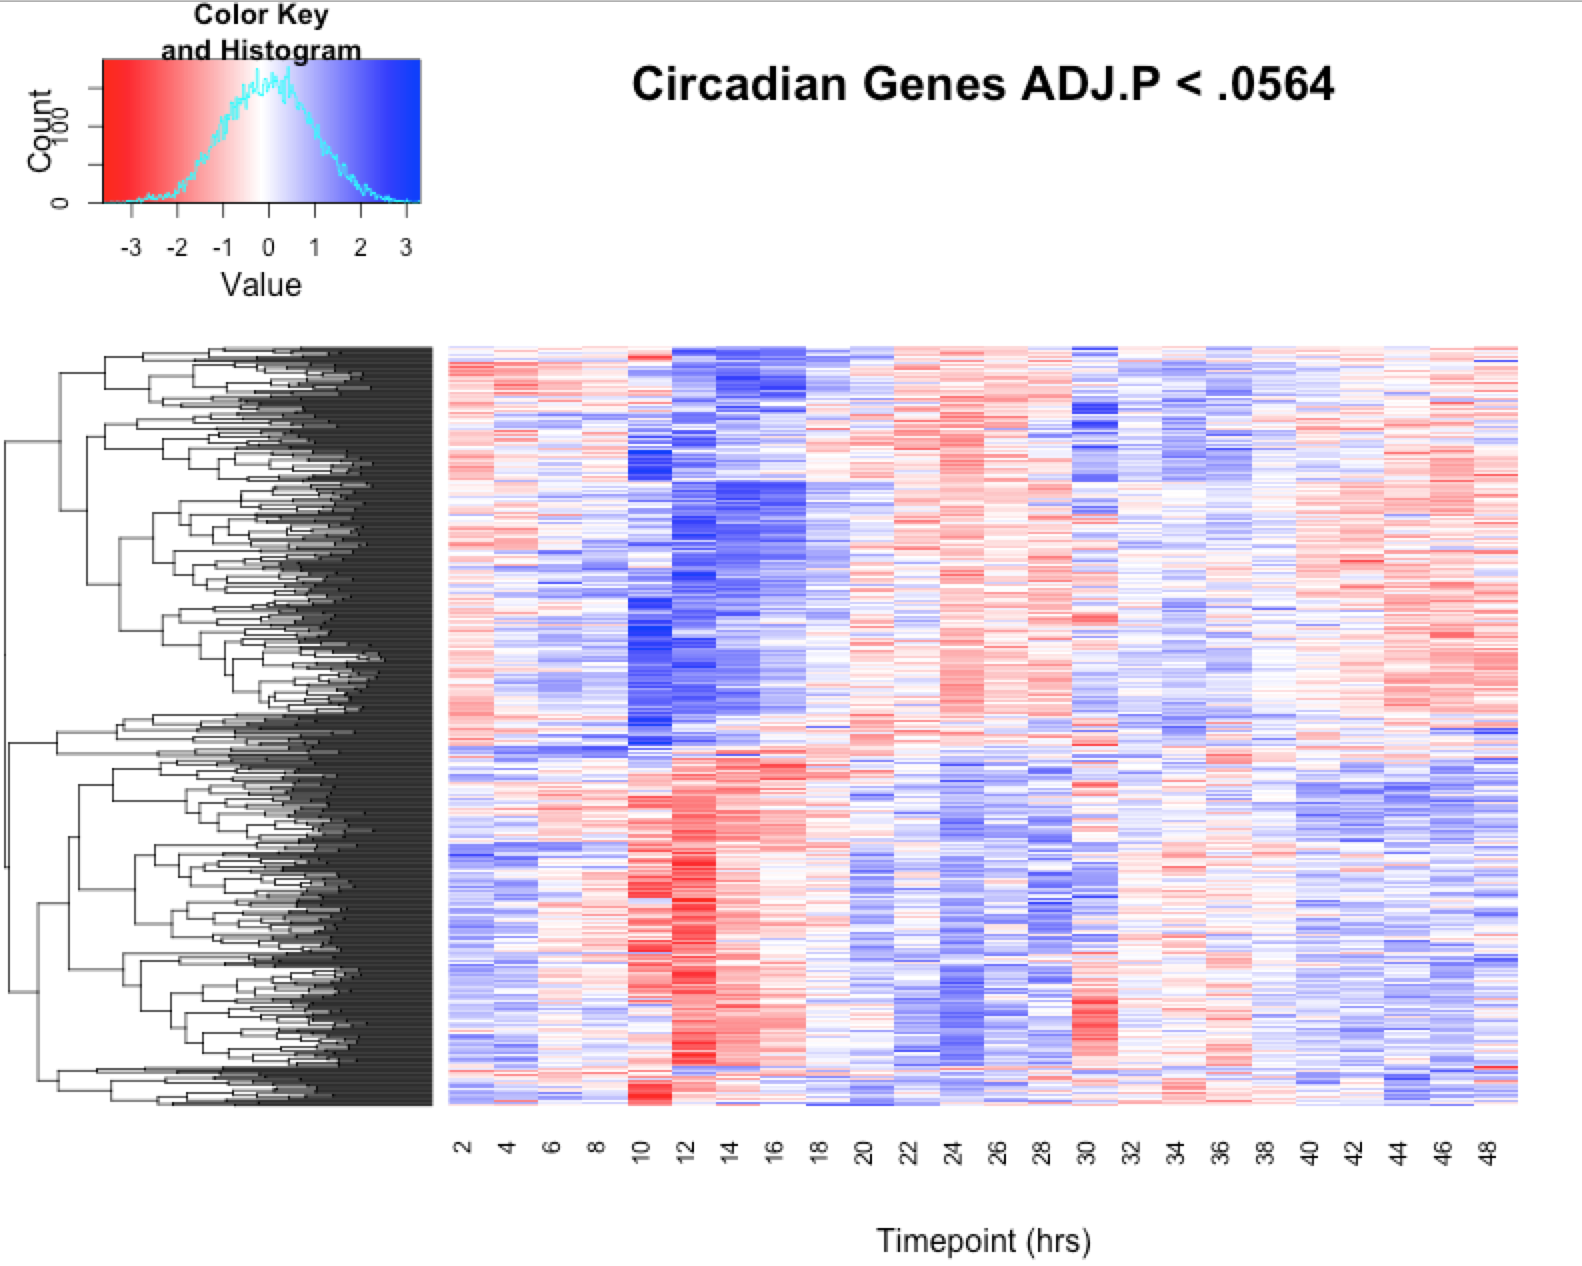
\includegraphics[width=.4\textwidth]{Circadian.png}\quad
  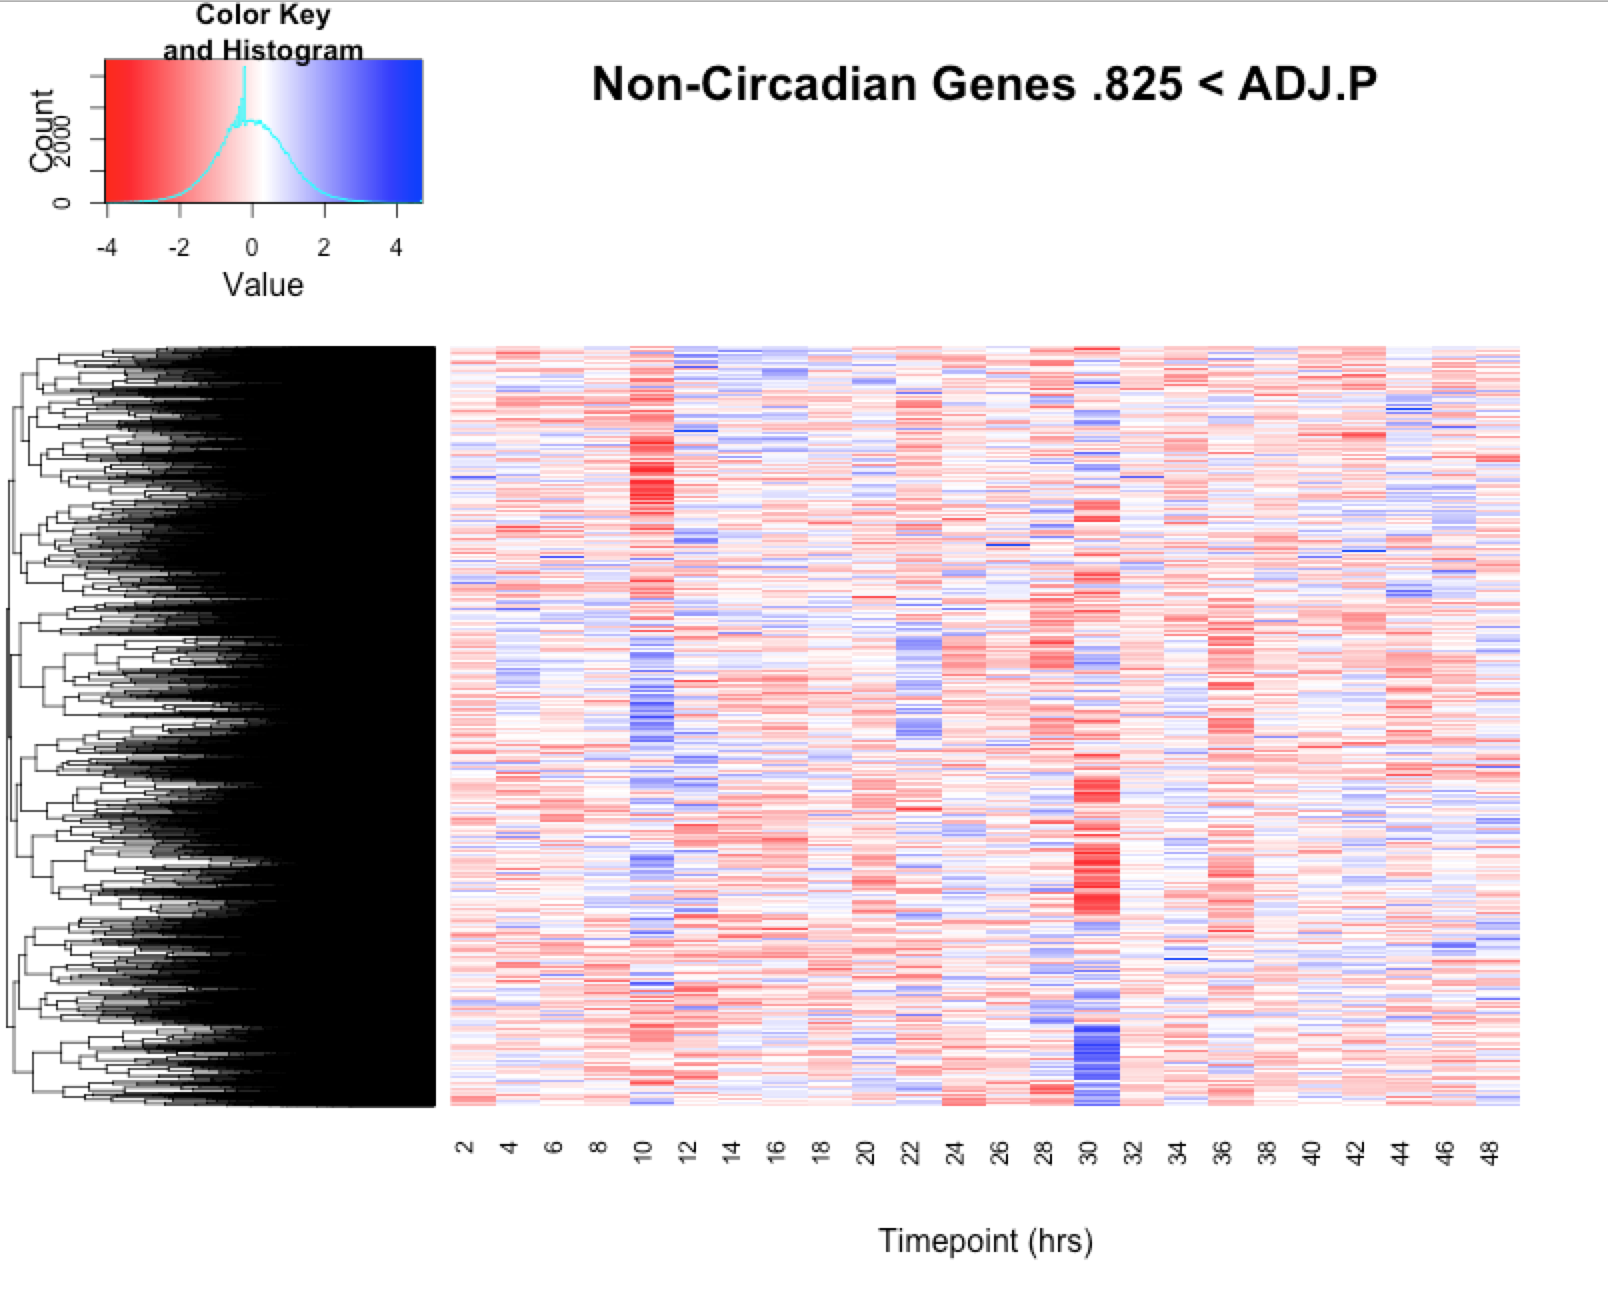
\includegraphics[width=.4\textwidth]{Non-Circadian.png}\\
  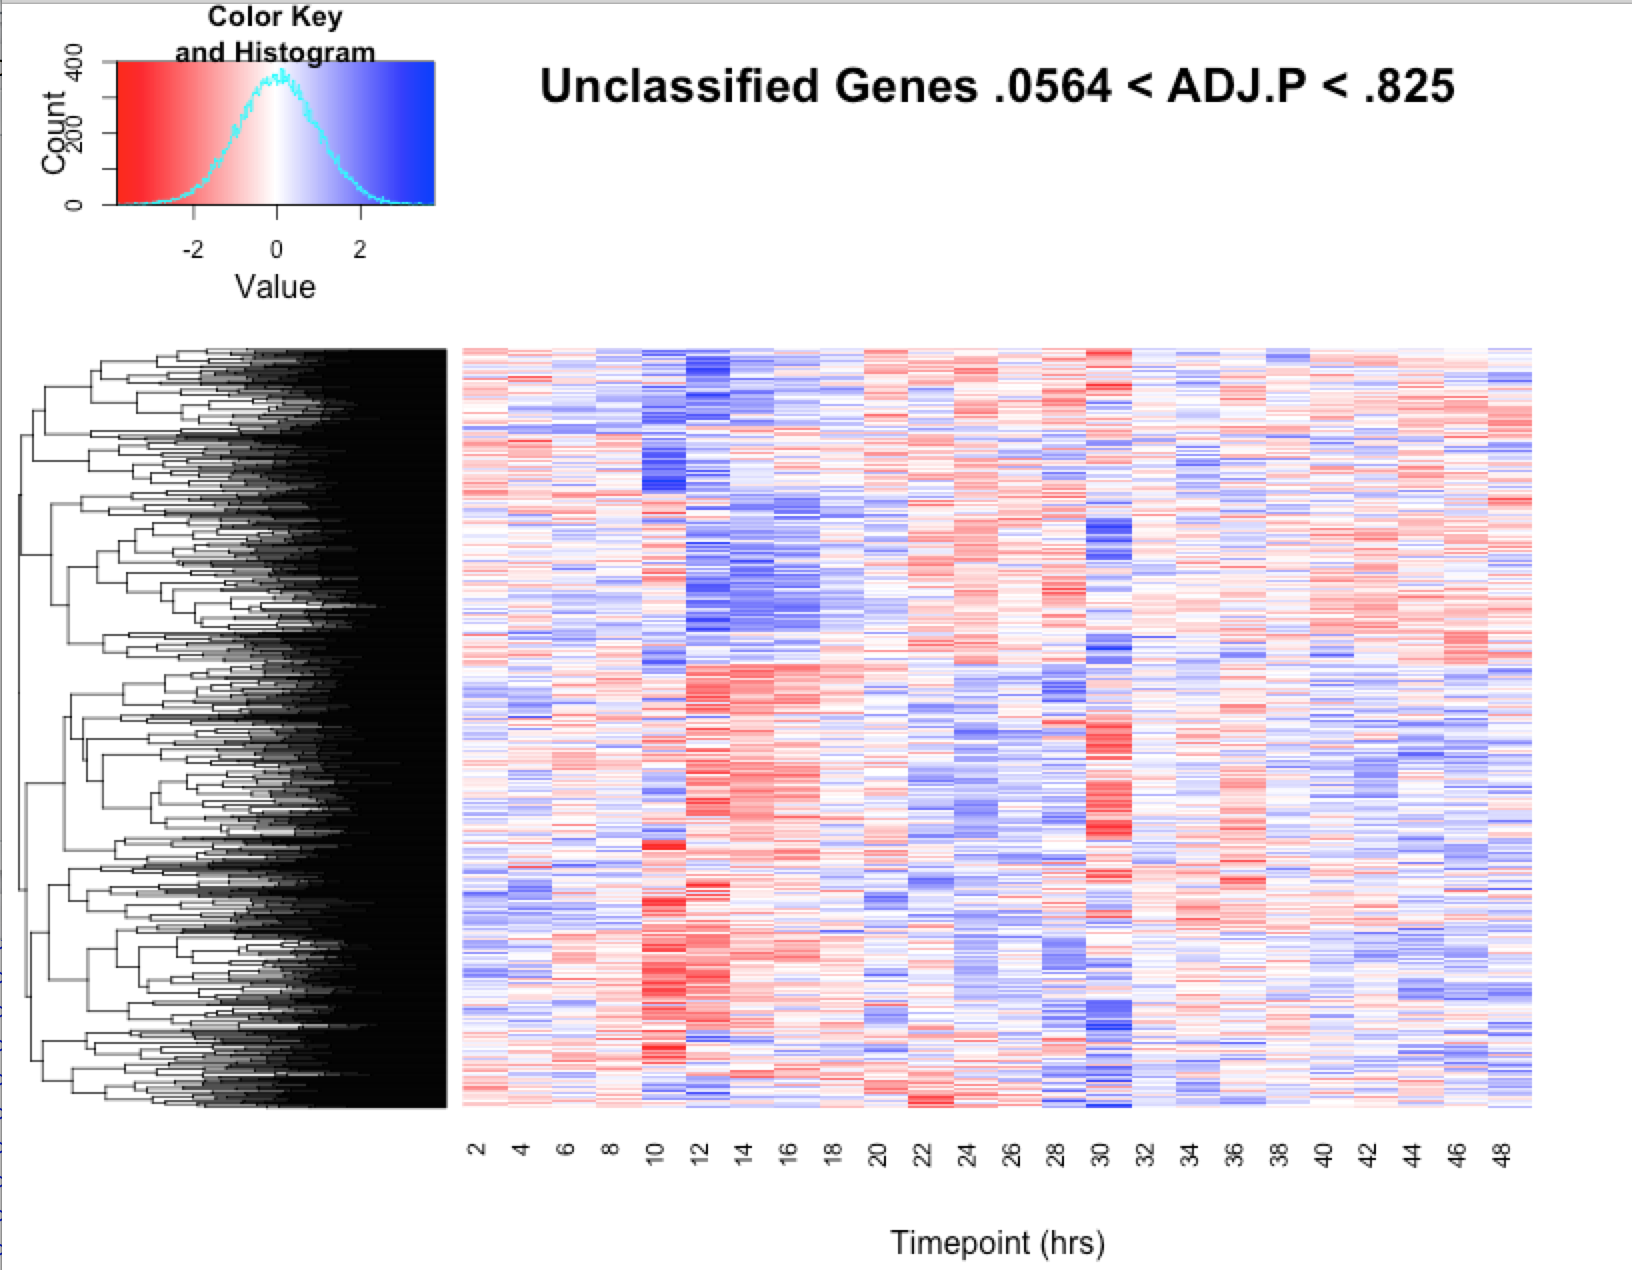
\includegraphics[width=.4\textwidth]{Unclassified.png}\quad
  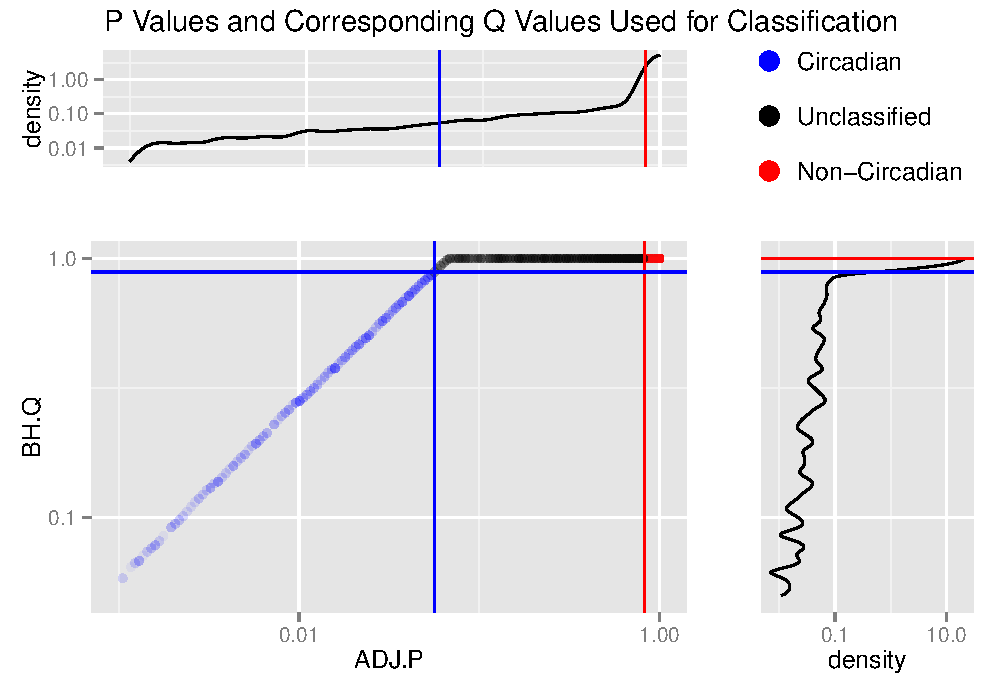
\includegraphics[width=.4\textwidth]{PvsQ.pdf}
  \caption{Hierarchically clustered heatmaps of each class along with a plot of P vs Q for all genes}
  \label{fig:1}
\end{figure*}

The training dataset employed in this project was derived from Neurospora Crassa a filamentous fungus which is one of the primary model organisms in the study of circadian clocks due to it's genetic tractability, ease of culture and possession of a semantically similar clock to higher eukaryotes.  All samples were synchronized with a light to dark transition and three biological replicates were collected every two hours for 48 hours.  These samples were then sequenced and aligned to the neurospora genome using tophat.  Feature counting was performed with HTSeq count and normalization performed with the DESeq bioconductor package.  The resulting gene counts were then processed using JTK for Circadian classification.  The training data is comprised of a combination of the normalized gene counts at each timepoint and a classifier of circadian, non-circadian or unclassified based on the adjusted P value output by JTK. The cutoffs for these classifiers were determined by examining the P and Q value distributions for all genes along with hierarchically clustered heatmaps for each set.

After processing our training data consists of 9548 temporal gene expression profiles, each one a $24-$dimensional vector. The data is divided into three classes, $\{\text{Circadian},\text{Unclassified},\text{Non-circadian}\}$. The unclassified data has some oscillatory behavior, but doesn't have a high enough $q-$value to be considered circadian. Non-circadian data is non-oscillatory. 

One of the main problems that needs to be addressed is how to deal with the vast difference in class volumes. Proposals that seem likely to work are data perturbation and data genesis via PCA. The latter would require doing a PCA analysis of each class to determine the eigen genes in each class, and then creating new linear combinations of them with predetermined monotonically decreasing component weights. 

The latter, data perturbation, would require determining some perturbation parameter, $\epsilon$, and using it to perturb data vectors with random numbers drawn from a Gaussian distribution, arranged in a diagonal matrix, $\textbf{G}$.:
\ee{
\vc{x}' =(\mathbb{1}+\epsilon\textbf{G} )\cdot\vc{x}
} 
To ensure that the perturbations are not too large, the analysis described in the first paragraph can then be utilized to determine the $q$-values of the new data. In this way we can supplement known data with synthetic data and balance the class volumes. 

\section{Experiment}



For the preliminary experiments that have been done we have made the following architectural choices:
\begin{itemize}
\item Activation Function - Sigmoid, with a soft max output layer
\item Error Function - Cross Entropy
\item Regularizor - Weight Penalization
\item Momentum - .1
\item Weight Decay - .001
\item Learning Rate - .1
\item Layer - {24-24-3, 24-48-3, 24-48-24-3, 48-96-3, 24-24-24-24-3, 24-48-24-24-3, 24-48-3-48-3 } 
\end{itemize}
Our main goal in the preliminary experiments was to determine the optimal number, and size, of the hidden layers in the ANN. Future expriments will explore changes in the other parameters of the network. 
\section{Conclusion}


\section{Algorithms}

\begin{algorithm}[H]
\caption{Feed Forward}\label{feed_forward}
\begin{algorithmic}[]
\Procedure{FeedForward}{$\vc x^{(0)}$,\textbf{W}}\\
\State $L \gets \text{number of layers in }\textbf{W}$
\State $N_l \gets \text{number of perceptrons in } \textbf{w}^{(l)}\in\textbf{W}$
\State $N_0 \gets \text{dim(domain(}(\vc x^{(0)})$\\

\State \textbf{for} $l=1,2,\dots,L$
\State \hspace{.25cm}$x^{(l-1)}_0 \gets 1$
\State \hspace{.25cm}\textbf{for} $i=1,2,\dots,N_l$
\State \hspace{.25cm}\hspace{.25cm}$x^{(l)}_i\gets\theta(\sum_{j=0}^{N_{l-1}}w^{(l)}_{ij}x^{(l-1)}_j)$\Comment{ and store}
\State \hspace{.25cm}\textbf{end}
\State \textbf{end}\\

\State \textbf{return} \textbf{X}$=(\vc x^{(0)},\vc x^{(1)},\dots,\vc x^{(L)})$\\
\EndProcedure
\end{algorithmic}
\end{algorithm}

\begin{algorithm}[H]
\caption{Back Propogation}\label{back_prop}
\begin{algorithmic}[]
\Procedure{BackProp}{\textbf{X}, $\vc y$, \textbf{W}}\\
\State $L \gets \text{number of layers in }\textbf{W}$
\State $N_l \gets \text{dimensionality of each } \vc x^{(l)} \in \textbf{X}$\\

\State \textbf{for} $l=L,L-1,\dots,,2,1$
\State \hspace{.25cm}\textbf{for} $i = 1,2,\cdots, N_l$
\State \hspace{.50cm}\textbf{if} $l=L$
\State \hspace{.75cm} $\delta^{(l)}_i \gets \phi(x_i^{(l)})\nabla_i E$
\State \hspace{.50cm}\textbf{else}
\State \hspace{.75cm} $\delta^{(l)}_i\gets \phi(x^{(l)}_i)\sum_{j=0}^{N_{l+1}}\delta^{(l+1)}_jw^{(l+1)}_{ji}$
\State \hspace{.50cm}\textbf{end}
\State \hspace{.50cm}\textbf{for} $j=1,2,\dots,N_{l-1}$
\State \hspace{.75cm}$w^{(l)}_{ij}\gets w^{(l)}_{ij}-\eta\left(\nabla^{(l)}_{ij}R+\delta^{(l)}_ix^{(l-1)}_j\right)$
\State \hspace{.50cm}\textbf{end}
\State \hspace{.25cm}\textbf{end}
\State \textbf{end}\\

\State \textbf{return} \textbf{W}\\
\EndProcedure
\end{algorithmic}
\end{algorithm}

\begin{algorithm}[H]
\caption{Train Network}\label{train_ANN}
\begin{algorithmic}[]
\Procedure{Train}{$\mathcal{D}$, \textbf{W}, numEpochs}\\

\State \textbf{for} $i = 1, 2, \dots,$ numEpochs
\State \hspace{.25cm} $\textbf{randomize}(\mathcal{D})$ 
\State \hspace{.25cm} $\textbf{for } d\in\mathcal{D}$
\State \hspace{.50cm} $\textbf{X} \gets \text{FeedForward}(d_1,\textbf{W})$
\State \hspace{.50cm} $\textbf{W} \gets \text{BackProp}(\textbf{X}, d_2,\textbf{W})$
\State \hspace{.25cm} \textbf{end}
\State \textbf{end}\\

\State \textbf{return W}\\

\EndProcedure
\end{algorithmic}
\end{algorithm}

\begin{algorithm}[H]
\caption{Cross Validation}\label{cross_val}
\begin{algorithmic}[]
\Procedure{CrossVal}{$\mathcal{D}$, \textbf{W}, numEpochs, N}\\

\State \textbf{randomize}$(\mathcal{D})$
\State \textbf{partition} $\mathcal{D}=\mathcal{D}^1\sqcup\mathcal{D}^2\sqcup\dots\sqcup\mathcal{D}^N$
\State \textbf{for } $i=1,2,\dots,N$
\State \hspace{.25cm} $\textbf{W}\gets \text{Train}(\mathcal{D\backslash \mathcal{D}}^i, \textbf{W}, \text{numEpochs})$
\State \hspace{.25cm} MSE$_i\gets\|\mathcal{D}^i_2-\text{FeedForward}(\mathcal{D}^i_1,\textbf{W})\|_2$
\State \textbf{end}
\State CVerror $\gets \text{mean}(\{MSE_i\})$\\
\State \textbf{return} CVerror\\

\EndProcedure
\end{algorithmic}
\end{algorithm}

\section{Bibliography}
\bibliographystyle{unsrt}
\bibliography{bibliography}


\end{document}